\chapter{Fundamentals}\label{chapt:basics}

\vspace{-1.5cm}

\section{Memory Hierarchy}\label{subchap:memhierarch}

The rate at which the processor speed develops is significantly faster than the development of the memory speed. This is known as the \textit{Memory Wall effect}. \cite{lwn_caches} \cite{memwall} This is a problematic development because in the worst case, if the two speeds strongly deviate from each other, the total speed of execution depends entirely on the slower speed, i.e. the memory speed. 

This slow development of memory speed in contrast to the processor speed is due to the design constraints of memory: capacity versus speed versus cost. One could adapt the memory speed to the processor speed, but would have to calculate with higher costs per bit. \cite[p. 124]{computerarch}

Despite this, in order to still meet the needs for cheap high capacity memory and simultaneously having high speed memory without increasing the total cost too much, different memory types are built and used together. These can be displayed in a so-called \textit{memory hierarchy}, which can be seen in figure \ref{fig:memhierarch}. \cite[p. 124-125]{computerarch}

The further down the hierarchy the memory is placed in figure \ref{fig:memhierarch} the cheaper the bit, the larger the memory capacity, the larger the memory access time, the lower the frequency of accessing by the processor and the farther away the memory is from the processor. \cite[p. 78]{quantivapproach}  \cite[p. 124-125]{computerarch}  Typical values for different levels can be seen in table \ref{table:memhierarch}. 

The benefit of this memory hierarchy design lies in the heuristic of \textit{principle of locality}. This heuristic states that a program typically accesses data that is located near previously accessed data, known as \textit{spatial locality}, or data that has been recently accessed, known as \textit{temporal locality}. \cite[p. 234]{threeeasy} \cite[p. 158-160]{computerarch}

\begin{figure}[H]
    \centering
    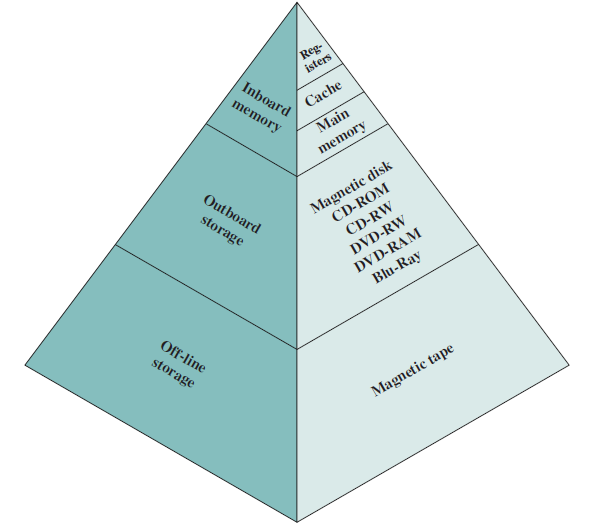
\includegraphics[width=.6\textwidth]{images/3_basics/mem-hierarch.png}
    \caption{Memory hierarchy\\Source: \cite[p. 125]{computerarch}}
    \label{fig:memhierarch}

\end{figure}


\begin{table}[H]
    \centering
    \renewcommand\tabularxcolumn[1]{m{#1}}
    \begin{tabularx}{\textwidth}{XXXXX}
    \hline
        \textbf{Level} & \textbf{1} & \textbf{2} & \textbf{3} & \textbf{4} \\ \hline
        Name & Registers & Cache & Main Memory & Disk Storage \\ \hline
        Typical Size & <4KiB & 32 KiB to 8 MiB  & <1 TB  & >1 TB \\ \hline
        Used\newline Technology & CMOS & CMOS SRAM & CMOS DRAM & Flash, Magnetic Disk \\ \hline
        Access time (ns) &  0.1–0.2  & 0.5–10  & 30–150  &  5,000,000 \\ \hline
        Frequency (MHz) & 10000-5000 & 2000-100 & 33-6 & 0.0002 \\ \hline
        Bandwidth (MiB/sec)  & 1,000,000–10,000,000  &  20,000–50,000  &  10,000–30,000  & 100–1000 \\ \hline
    \end{tabularx}
    \caption{Typical values for the different memory levels\\Source: \cite[p. 3]{quantivapproach-ApB}}
    \label{table:memhierarch}
\end{table}

The memory hierarchy design takes advantage of this principle by organizing data in different levels of the hierarchy based on their access patterns, with the faster and smaller memory closer to the processor and the slower and larger memory further away. This allows for faster and more efficient access to frequently accessed data, while less frequently accessed data can be stored in slower and larger memory. \cite[p. 127]{computerarch}

\section{Caches}

Level two memory in the memory hierarchy, or cache, is a small capacity memory which buffers a limited amount of recently accessed memory references. \cite[p. 94]{threeeasy} \cite[p. 23]{brendan}

When the processor loads a memory location, whether code or data, it first looks in the cache to see if it is already stored there. If it is in the cache, the processor fetches the information from the cache. This is called a cache hit. If the processor does not find it in the cache, the information has to be retrieved from main memory or the disk, which takes much longer than accessing the cache. This is called a cache miss. \cite[p. 2]{quantivapproach-ApB} \cite[p. 128]{computerarch}

% This is because the memory bandwidth increases as the numbers of cores grows.
Nowadays, the level two memory in the memory hierarchy no longer consists of a single cache but of a multilevel cache schema. The first-level cache can be designed to match the fast clock cycle time of modern processors, while the higher-level caches can be designed to have a larger capacity to store a significant amount of data from the main memory. This helps to reduce the number of times that the processor has to access the slower main memory. \cite[p. 78-83]{quantivapproach} 

The caches can be located either internally on the CPU die or externally. The exact depth, capacity and distribution of the caches depends on its type and model. \cite[p. 231-232]{brendan} An example can be seen in figure \ref{fig:cachehierarch}.

% In addition, logic density has increased over the years, allowing the cache to be on the same chip as the processor. Being on the same chip allows the cache to have its own bus with shorter data paths that are decoupled from the external bus. This reduces pressure on the external bus, which is shared with other components, and cache access time. \cite{computerarch} 

\vspace{.5cm}
\begin{figure}[H]
    \centering
    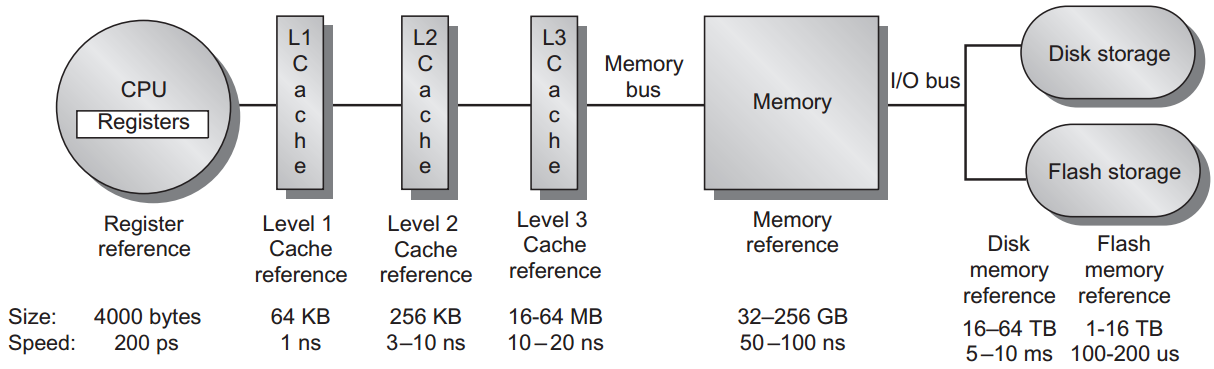
\includegraphics[width=\textwidth]{images/3_basics/caches.png}
    \caption{Memory hierarchy for an example server\\Source: \cite[p. 79]{quantivapproach}}
    \label{fig:cachehierarch}
    \vspace{-\baselineskip}
\end{figure}

Furthermore, individual caches can be split into separate instruction and data caches instead of a single unified cache. The trend is toward splitting the L1 cache into an instruction L1 cache (IL1 cache) and a data L1 cache (DL1 cache) and using a unified cache for higher levels. \cite[p. 149]{computerarch} 

The advantage of a split in the L1 cache is that it eliminates the contention between different units for a single cache in the pipeline. The disadvantage is that two caches have to be implemented instead of a single unified cache, which is more expensive. \cite{cache_memory} \cite[p. 147-149]{computerarch}

\section{Virtual Memory}\label{section:vm}

Virtual memory is an abstraction provided by the hardware to the processor. The operating system, which sets up and manages the virtual memory space for each process, enables the process to have its own virtual address space that maps to physical memory as needed. \cite[p. 133-134]{threeeasy} \cite[p. 194-195]{tanenbaum}

The addresses in this address space are so called \textit{virtual addresses}, which must be converted to the true \textit{physical memory address} before a memory access. This is called \textit{address translation}. It should be noted that this needs to be done for \textbf{all} processes and \textbf{every} memory access, in other words every time for example an instruction is loaded and executed in a program or the kernel. \cite[p. 133-134]{threeeasy} \cite[p. 195-196]{tanenbaum}

With this methodology, the kernel has the freedom to choose dynamically any memory place in physical memory for an address space which best suits the used memory layout scheme. \cite[p. 133]{threeeasy} \cite[p. 190-191]{tanenbaum}

Additionally, multiple virtual addresses in multiple processes can point to the same \textit{physical address}, such as for example in the case of shared libraries. Furthermore, the processes are protected from other processes, since the illusion prevails that they only run for themselves and use their own address space. \cite[p. 192, 137-138]{threeeasy} \cite[p. 228-230]{tanenbaum}

\section{Paging}\label{section:page}

Most virtual memory systems structure the memory in addition in the form of \textit{pages}. \textit{Pages} are chunks of memory of a program which are mapped to chunks of physical memory, called \textit{page frames}. \cite{virtual-memory} \cite[p. 195-196]{tanenbaum} The methodology of virtual memory in combination with paging can be seen in figure \ref{fig:singlepage} and \ref{fig:pagephysical}.

\begin{figure}[H]
     \centering
     \captionsetup{justification=raggedright}
     \begin{minipage}[b]{0.4\textwidth}
         \centering
         \hspace*{5mm}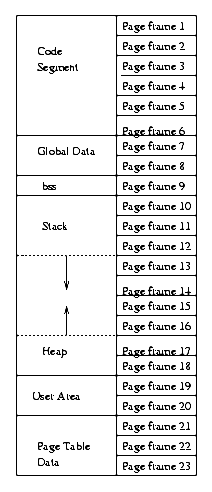
\includegraphics[height=8.5cm]{images/3_basics/pages-single.png}
         \caption{Address space of an example ELF file split in pages Source: \cite{pic:singlepage}}
         \label{fig:singlepage}
     \end{minipage}%
     \hspace*{7mm}
     \begin{minipage}[b]{0.6\textwidth}
         \centering
         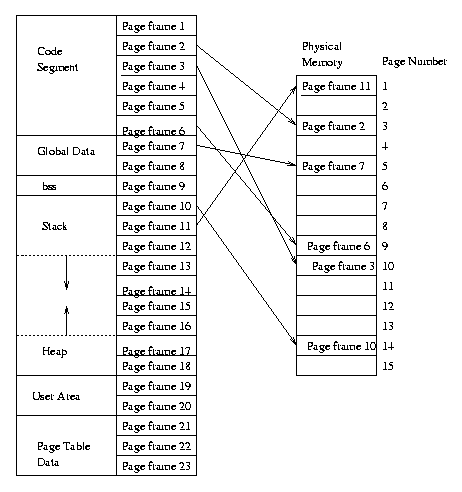
\includegraphics[width=.85\textwidth]{images/3_basics/pages-with-physical.png}
         \caption{Schematic representation of connections between virtual and physical pages\\
         Source: \cite{pic:singlephysical}}
         \label{fig:pagephysical}
     \end{minipage}
\end{figure}    
\vspace{-\baselineskip}

An advantage of this combination is that the kernel can load a physical address at a later point in time in order not to fill the physical memory prematurely and to leave free memory for other programs. This is called \textit{demand paging}. \cite[p. 240]{threeeasy} \cite[p. 299]{computerarch}

This information, which virtual page points to which physical page, is called a \textit{page table entry} (PTE). The kernel stores every PTE of every program combined in a \textit{page table}. In addition, a PTE stores more than the address translation. It also stores additional information like a valid bit, protection bits, \textit{present bit}, etc. \cite[p. 172-174]{threeeasy} \cite[p. 199-200]{tanenbaum}

The \textit{present bit} indicates whether the page has already been loaded into physical memory or not. If this has not happened at the time of the memory access, a \textit{page fault} is invoked and the page is loaded into physical memory from other storage, for example the hard drive.  \cite[p. 174]{threeeasy} \cite[p. 200]{tanenbaum}
\enlargethispage{\baselineskip}

Besides processing the address translation and other information bits in the PTE, the page table must first be looked through in order to find the entry for the virtual page. Searching the page table is also called \textit{page table walking}. \cite[p. 187]{threeeasy} \cite[p. 204-205]{tanenbaum}

\newpage

Instead of a simple linear page table, which is a simple list structure of all the PTEs, nowadays \textit{multi-level page tables} are used to reduce the size of the page table to be stored per process. This is also called a \textit{page directory}. However, this has the disadvantage that a multi-level page table is more complex to keep track of and look through when searching for a PTE than a linear page table. \cite[p. 205-207]{threeeasy} \cite[p. 205-207]{tanenbaum}

In order to relieve the processor of all this additional work, an extra hardware unit was designed that is dedicated to this task: the \textit{Memory Management Unit} (MMU). \cite[p. 135]{threeeasy} \cite[p. 195-196]{tanenbaum}\\
Figure \ref{fig:simplemmu} shows the positioning of the MMU in comparison to other components.

\begin{figure}[H]
    \centering
    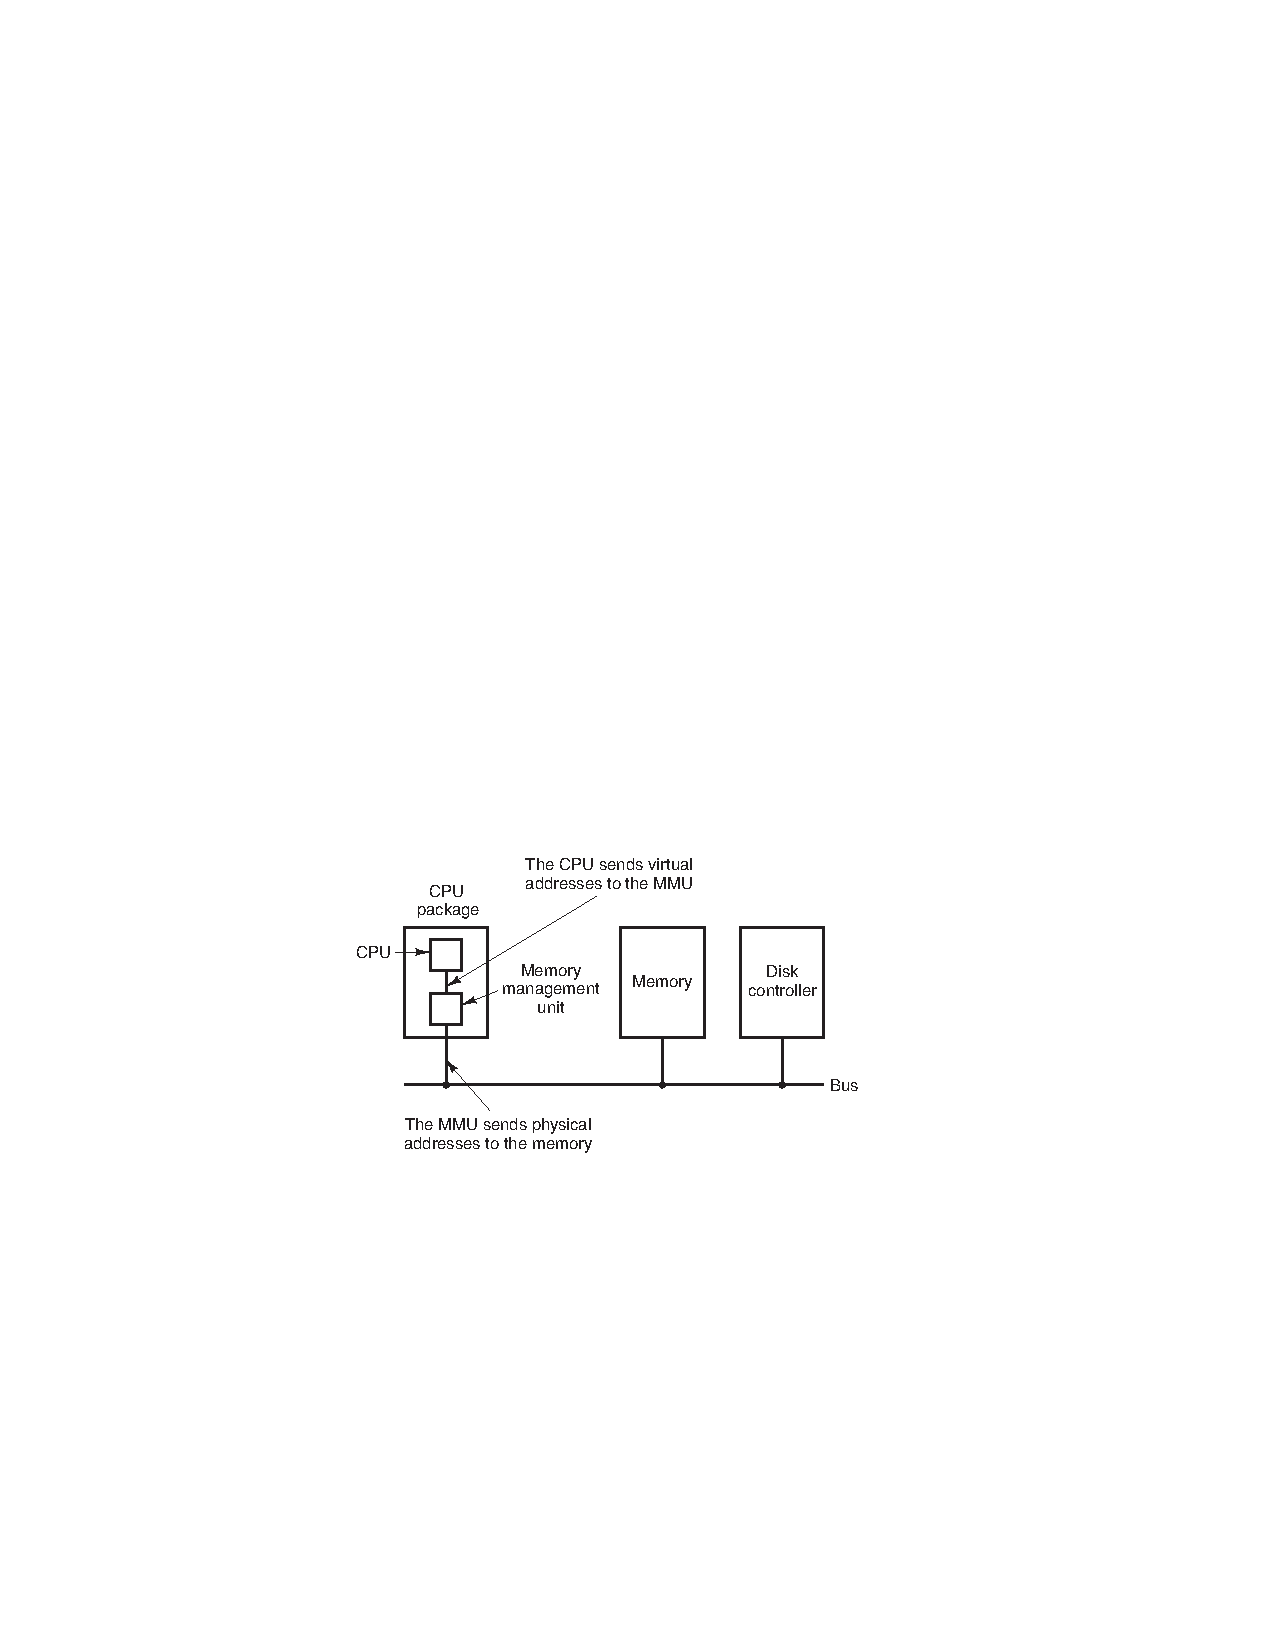
\includegraphics[width=.65\textwidth]{images/3_basics/hardware-paging.pdf}
    \caption{Hardware positions and connections\\Source: \cite{tanenbaum}}
    \label{fig:simplemmu}
\end{figure}
\vspace{-\baselineskip}

\section{Translation Lookaside Buffer (TLB)}\label{section:tlb}

To further speed up the address translation, a hardware cache was introduced that temporarily stores frequently accessed PTEs for use in the near future. This cache is located in the MMU itself and is called \textit{translation lookaside buffer}, or \textit{TLB} for short. It is a small cache which stores only a small amount of entries. \cite[p. 183]{threeeasy} \cite[p. 202]{tanenbaum}

When a memory access takes place, the MMU checks first the TLB to see if the desired PTE already exists in the TLB. If this is the case, a so called \textit{TLB hit}, the desired PTE is returned to the process. \cite[p. 184]{threeeasy} \cite[p. 203]{tanenbaum}

If this is not the case, the MMU starts the process of page table walking and, in the worst case, page faulting. This case is called a \textit{TLB miss}.  \cite[p. 184]{threeeasy} \cite[p. 204]{tanenbaum} If this happens multiple times because, for example, the cache full is or the wrong PTEs were stored, then one speaks of \textit{TLB pressure}.

Since the entries in the TLB are cached for the most frequently accessed PTEs per process, it is important to be careful that a process is not misinterpreting the remaining entries in the TLB by another process if a process switch happens. The simplest way to avoid this problem is to flush the entire TLB when a process changes, which is called \textit{TLB flush}. \cite[p. 191-192]{threeeasy} \cite{lwn_vm} \cite[p. 233-234]{tanenbaum} The entire process is illustrated in figure \ref{fig:memstatemachine} and \ref{fig:memaccesstime}.

\begin{figure}[H]
    \centering
    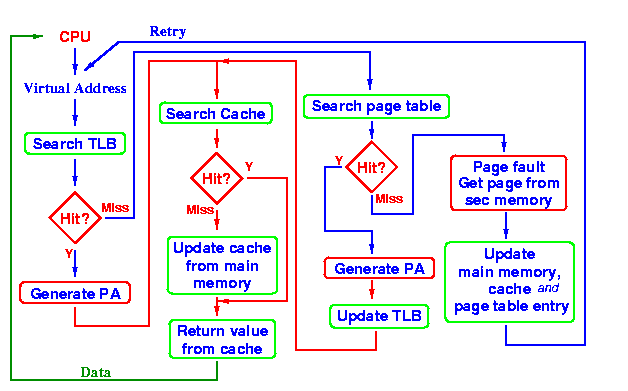
\includegraphics[width=.8\textwidth]{images/3_basics/mem_op.png}
    \caption{Flowchart of a memory access\\Source: \cite{pic:memop}}
    \label{fig:memstatemachine}
\end{figure}
\vspace{-\baselineskip}

Additionally, figure \ref{fig:memaccesstime} shows a more broken down example with additional approximate time sequences. From this schematic one can see that in the process of memory access through the MMU, page faults should be avoided as much as possible, because this leads to additional waiting times, especially if they occur frequently.

In modern systems, to profit from the principle of locality, the TLB is split in \textit{Instruction Translation Lookaside Buffer} (ITLB) and \textit{Data Translation Lookaside Buffer} (DTLB). \cite[p. 2, 4-5]{quantivapproach-ApL}

\vspace{\baselineskip}
\begin{figure}[H]
    \centering
    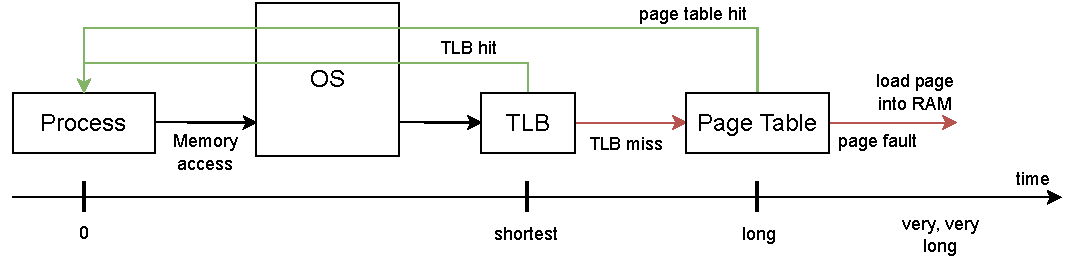
\includegraphics[width=\textwidth]{images/3_basics/mmu-more.pdf}
    \caption{Simple schematic of a memory access with time axis}
    \label{fig:memaccesstime}
\end{figure}
\vspace{-\baselineskip}

ITLB and DTLB are separated because instructions and data have different access patterns. Instructions are typically read sequentially, with the next instruction being located at a memory address that is close to the current instruction. On the other hand, data access patterns can be more random, with data being accessed from various locations and with random size in memory. \cite[p. 4-5]{quantivapproach-ApL}

\section{Performance Monitoring Unit (PMU)}\label{section:pmu}

The \textit{Performance Monitor Unit} (PMU) is a hardware component in modern computer processors that is used to measure various performance-related metrics such as the number of retired instructions executed, the number of cache misses, the number of branch mispredictions, etc. \cite[p. 156]{brendan} \cite{pmushort}

The PMU can be accessed by software through a set of registers which are used to configure the counters, read their values and calculate specific performance metrics like \textit{instructions per cycle} (IPC). \cite{how-counters-work} \cite[p. 681]{brendan} \cite{pmushort}

Depending on the processor model other features could be included like \textit{Last Branch Recording} (LBR), \textit{Event-Based Sampling} (EBS), \textit{Precise Event-Based Sampling} (PEBS) and other. \cite[p. 43]{patmc} The Linux kernel uses its own frontend tool \textit{perf}, which is an easy to use interface to access and configure the counters of the PMU. \cite[p. 671]{brendan}